\chapter{Background}

This section presents a block diagram of a proof-of-concept system and introduces many of the concepts and motivations involved in understanding each block.

\section{System overview}

A block-diagram of the proof-of-concept system is illustrated in [Figure X]. The system is separated into two parts: the sensor module (consisting of image sensor and encoder FPGA) and the camera mainboard (with the approrpriate decoder FPGA).

[Insert system block diagram here]

\section{Field-Programmable Gate Arrays}

\subsection{Hardware Description Languages}
\subsection{Synthesis and Place-and-Route}

\section{CCD and CMOS sensor technologies}

The sensors themselves fall into one of two categories depending on technology used: \gls{ccd} and \gls{cmos}. While both use an array of photosites to collect charge from incident photons during exposure time, the readout and analogue-to-digital conversion process differs for each. During readout time, \glspl{ccd} sequentially shift the accumulated charges into horizontal and vertical readout registers where they are transferred to a chip-level output amplifier and analogue-to-digital converter to generate a binary bitstream. \gls{ccd} image sensors are capable of very low noise and high sensitivity due to the use optimised photosites; this made them a very popular choice for applications demanding high image quality.

Unlike \glspl{ccd}, which rely on a very specialised fabrication process, CMOS sensors can be manufactured using traditional \gls{cmos} processes, benefiting greatly from the associated economies of scale. \gls{aps}, the most common form of \gls{cmos} sensor, differ from \glspl{ccd} in that each photosite contains a dedicated amplifier, meaning that the light-induced voltages can be driven directly to the row and column decoders for digitisation. Because of the \gls{cmos} fabrication process, other camera functions can also be integrated onto the same chip, cutting both the cost and size of the device \cite{10_ge_2012}.  This level of integration, and the faster speeds of parallel readout processing have meant that \gls{cmos} sensors have seen a recent surge in popularity, and are forecast to account for 85\% of the total image sensor market in 2017 \cite{11_ic_insights_2013}.

\begin{figure}
  \centering
  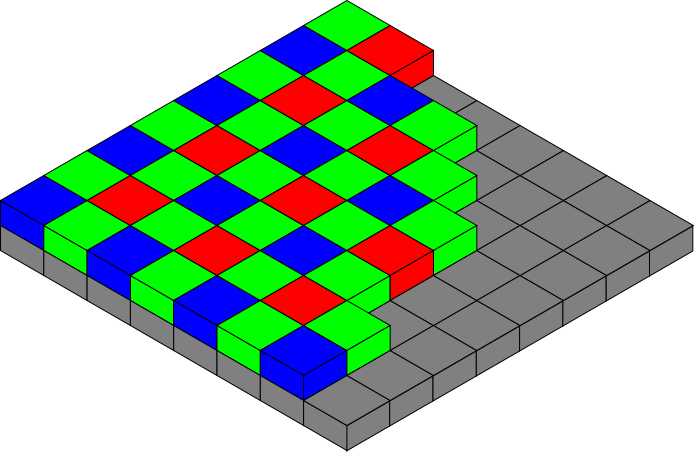
\includegraphics[width=1\textwidth]{./img/bayer_pattern.png}\par
Source: diagram by Cburnett, distributed under CC BY-SA 3.0
  \caption{Bayer filter}
  \label{fig:bayer_pattern}
\end{figure}

Photosites can only measure light intensity, not wavelength, producing greyscale images. By placing a coloured filter in front of each photosite, it is possible to only let light of a certain wavelength through \cite{12_eastman_kodak_company_1976}. Given the fixed pattern of the \gls{cfa}, it is possible to generate a full-colour image using a demosaicing algorithm, the simplest of which is bilinear interpolation, to calculate the red, green and blue intensities for each pixel \cite{13_malvar_he_cutler_2015}. One such \gls{cfa}, the Bayer filter, contains twice as many green elements as red and blue to mimic the physiology of the human eye, as illustrated in Figure \ref{fig:bayer_pattern}.